\documentclass[10pt]{article}
\usepackage[utf8]{inputenc}

\title{Algoritmos e Estruturas de Dados I}
\author{Paulo Lima}
\date{Abril 2019}


\usepackage{natbib}
\usepackage{graphicx}

\begin{document}

\maketitle
\newpage
\section{Introdução}
Estruturas de dados é o nome dado a organização de dados e algoritmos de forma coerente e racional de modo a otimizar o seu uso. De acordo com o modo como um conjunto de dados são organizados e como as operações que são efetuadas sobre estes dados pode-se solucionar de forma simples problemas extremamente complexos, como demonstrado no livro \cite{Estrutura}.

Existem diversos modelos de estruturas de dados, e novos modelos são criados constantemente pois acompanham também a evolução dos algoritmos e das linguagens de programação. Apresentar as diversas estruturas de dados fundamentais, como estruturas lineares (listas encadeadas, pilhas, filas, etc.), estruturas não-lineares (árvores), os algoritmos básicos para a sua manipulação, assim como as suas aplicações; Introduzir noções básicas de complexidade de algoritmos e técnicas básicas para comparação dos tempos de execução dos algoritmos estudados; Apresentar a importância da escolha da estrutura de dados e algoritmos adequados para a resolução de problemas de maneira eficiente.

É um dos temas fundamentais da ciência da computação, utilizado nas mais variadas áreas e para as mais variadas finalidades. No entanto para começarmos a entender o conceito devemos, antes entender o conceito de algoritmos, pois algoritmos manipulam dados.

Dados quando estão organizados de uma forma coerente representam uma estrutura de dados. Escolher uma estrutura de dados ideal pode tornar-se um problema difícil para uma determinada solução. As pesquisas e estudos das estruturas de dados estão em constante desenvolvimento, apesar disso, existem estruturas que têm se mostrado padrão, ou seja, são clássicas.

Estruturas de dados possuem características básica, no entanto finalidades bastante diversas, um tipo de estrutura de dados é a estrutura em pilhas, demonstrada da figura \ref{imagem}
\begin{figure}[h!]
    \centering
    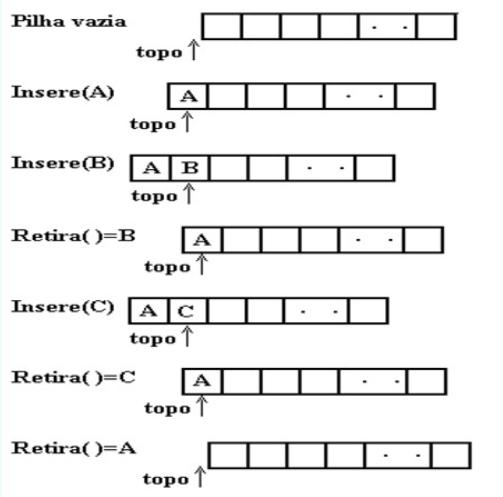
\includegraphics[scale=0.45]{Paulo_Kaynan.png}
    \caption{Estrutura de Pilhas}
    \label{imagem}
\end{figure}
\newpage

\section{Relevância}
Estrutura de dados e algoritmos são temas fundamentais da ciência da computação, sendo utilizados nas mais diversas áreas do conhecimento e com os mais diferentes propósitos de aplicação. Sabe-se que algoritmos manipulam dados. Quando estes dados estão organizados (dispostos) de forma coerente, caracterizam uma forma, uma estrutura de dados. A organização e os métodos para manipular essa estrutura é que lhe confere singularidade (e vantagens estratégicas, como a minimização do espaço ocupado na memória RAM), além (potencialmente) de tornar o código-fonte mais enxuto e simples. 

Com base no projeto pedagógico \cite{Projeto}. Pode-se considerar a tabela \ref{tabela} expressa de forma simples a importância de Estrutura de dados e algoritmos I, tendo em vista  que é pré-requisito para 12 outras disciplinas.
    


\begin{table}[]
\begin{tabular}{|l|l|}
\hline
\begin{tabular}[c]{@{}l@{}}CC0102\\ Introdução à Programação\end{tabular}                       & \begin{tabular}[c]{@{}l@{}}É PRÉ REQUISITO PARA ALGORITMO\\  E ESTRUTURA DE DADOS\end{tabular}     \\ \hline
\begin{tabular}[c]{@{}l@{}}CC0301\\ Algoritmos e Estruturas de \\ Dados II\end{tabular}         & \begin{tabular}[c]{@{}l@{}}TEM ALGORITMO E ESTRUTURA \\ \\ DE DADOS COMO PRE REQUISTO\end{tabular} \\ \hline
\begin{tabular}[c]{@{}l@{}}CC0302\\ Laboratório de Programação\end{tabular}                     & \begin{tabular}[c]{@{}l@{}}TEM ALGORITMO E ESTRUTURA \\ \\ DE DADOS COMO PRE REQUISTO\end{tabular} \\
\hline
\begin{tabular}[c]{@{}l@{}}CC0401\\ Algoritmos em Grafos\end{tabular}                           & \begin{tabular}[c]{@{}l@{}}TEM ALGORITMO E ESTRUTURA \\ \\ DE DADOS COMO PRE REQUISTO\end{tabular} \\
\hline
\begin{tabular}[c]{@{}l@{}}CC0402\\ Programação Orientada a \\ Objetos\end{tabular}             & \begin{tabular}[c]{@{}l@{}}TEM ALGORITMO E ESTRUTURA \\ \\ DE DADOS COMO PRE REQUISTO\end{tabular} \\ \hline
\begin{tabular}[c]{@{}l@{}}CC0404\\ Programação Concorrente\end{tabular}                        & \begin{tabular}[c]{@{}l@{}}TEM ALGORITMO E ESTRUTURA \\ \\ DE DADOS COMO PRE REQUISTO\end{tabular} \\ \hline
\begin{tabular}[c]{@{}l@{}}CC0405\\ Fundamentos de \\ Linguagens \\ de Programação\end{tabular} & \begin{tabular}[c]{@{}l@{}}TEM ALGORITMO E ESTRUTURA \\ \\ DE DADOS COMO PRE REQUISTO\end{tabular} \\ \hline
\begin{tabular}[c]{@{}l@{}}CC0501\\ Projeto e Análise de A\\ lgoritmos\end{tabular}             & \begin{tabular}[c]{@{}l@{}}TEM ALGORITMO E ESTRUTURA \\ \\ DE DADOS COMO PRE REQUISTO\end{tabular} \\ \hline
\begin{tabular}[c]{@{}l@{}}CC0503\\ Banco de Dados\end{tabular}                                 & \begin{tabular}[c]{@{}l@{}}TEM ALGORITMO E ESTRUTURA \\ \\ DE DADOS COMO PRE REQUISTO\end{tabular} \\ \hline
\begin{tabular}[c]{@{}l@{}}CC0504\\ Sistemas O\\ peracionais\end{tabular}                       & \begin{tabular}[c]{@{}l@{}}TEM ALGORITMO E ESTRUTURA \\ \\ DE DADOS COMO PRE REQUISTO\end{tabular} \\ \hline
\begin{tabular}[c]{@{}l@{}}CC0601\\ Autômatos, Computabilidade \\ e Complexidade\end{tabular}   & \begin{tabular}[c]{@{}l@{}}TEM ALGORITMO E ESTRUTURA \\ \\ DE DADOS COMO PRE REQUISTO\end{tabular} \\ \hline
\begin{tabular}[c]{@{}l@{}}CC0602\\ Computação Gráfica\end{tabular}                             & \begin{tabular}[c]{@{}l@{}}TEM ALGORITMO E ESTRUTURA \\ \\ DE DADOS COMO PRE REQUISTO\end{tabular} \\ \hline
\begin{tabular}[c]{@{}l@{}}CC0701\\ Compiladores\end{tabular}                                   & \begin{tabular}[c]{@{}l@{}}TEM ALGORITMO E ESTRUTURA \\ \\ DE DADOS COMO PRE REQUISTO\end{tabular} \\ 
\hline

\label{tabela}
\end{tabular}
\end{table}


\newpage
\bibliographystyle{ieeetr}
\bibliography{Paulo_Kaynan.bib}
\cite{Projeto}
\cite{Estrutura}
\cite{Wiki}
\end{document}
